\documentclass[aspectratio=169]{beamer}

% Default packages
\usepackage[T1]{fontenc}
\usepackage[utf8]{inputenc}
\usepackage[english]{babel}
\usepackage{pgfplots}
\pgfplotsset{compat=newest}
\usepackage{booktabs}
\usepackage{siunitx}
\usepackage{caption}
\usepackage{subcaption}

% Font selection
% Latin Modern
\usepackage{lmodern}
% Verdana font type
%\usepackage{verdana}
% Helvetica
%\usepackage{helvet}
% Times (text and math)
%\usepackage{newtx, newtxmath}
% Nice font combination
%\usepackage{mathptmx} % math
%\usepackage{sourcesanspro} % sans-serif
\usepackage{charter} % serif

%\newcommand{\figurelabel}[1]{\vspace{1cm}\\\textbf{#1}}

% Use DTU theme, see below for options
\usetheme[department=compute]{DTU}

\title[DTU Templates]{Ruling out the Rulers}
\author{Mikkel Bjørn Goldschmidt\\Supervised by Professor Aasa Feragen \& PhD-student Manxi Lin}
\institute{DTU Compute}
\date{\today}
	
\newcommand{\tabitem}{{\color{dtured}$\bullet$} }

\begin{document}
\frame{
	\maketitle
}

\frame{
	\frametitle{Diagnosing skin lesions}
	% Insert some images of skin lesions here
	\textbf{Dataset}: HAM10000 (Human Against Machine)\\
	\vspace{1cm}

	\begin{columns}
		\begin{column}{0.4\textwidth}
			\includegraphics[width=\textwidth]{build/example_images/example_images.png}
		\end{column}
		\begin{column}{0.55\textwidth}
			\tiny
			\begin{table}[ht]
				\begin{center}
					\begin{tabular}{|c|c|c|c|c|c|c|}
						\hline
						Label & Name                          & Severity      & Dataset prevalence \\ \hline
						akiec & Bowens disease                & pre-malignant & $3.27\%$           \\ \hline
						nv    & Melanocytic nevi              & benign        & $66.94\%$          \\ \hline
						mel   & Melanoma                      & malignant     & $11.11\%$          \\ \hline
						bkl   & Benign keratosis-like lesions & benign        & $10.97\%$          \\ \hline
						bcc   & Basal cell carcinoma          & malignant     & $5.13\%$           \\ \hline
						vasc  & Vascular lesions              & benign        & $1.41\%$           \\ \hline
						df    & Dermatofibroma                & benign        & $1.14\%$           \\ \hline
					\end{tabular}
				\end{center}
				\vspace{1em}
				\textbf{Table 4.1}
			\end{table}
		\end{column}
	\end{columns}
}

\frame{
	\frametitle{The Clever Hans Phenomenon}
	\centering
	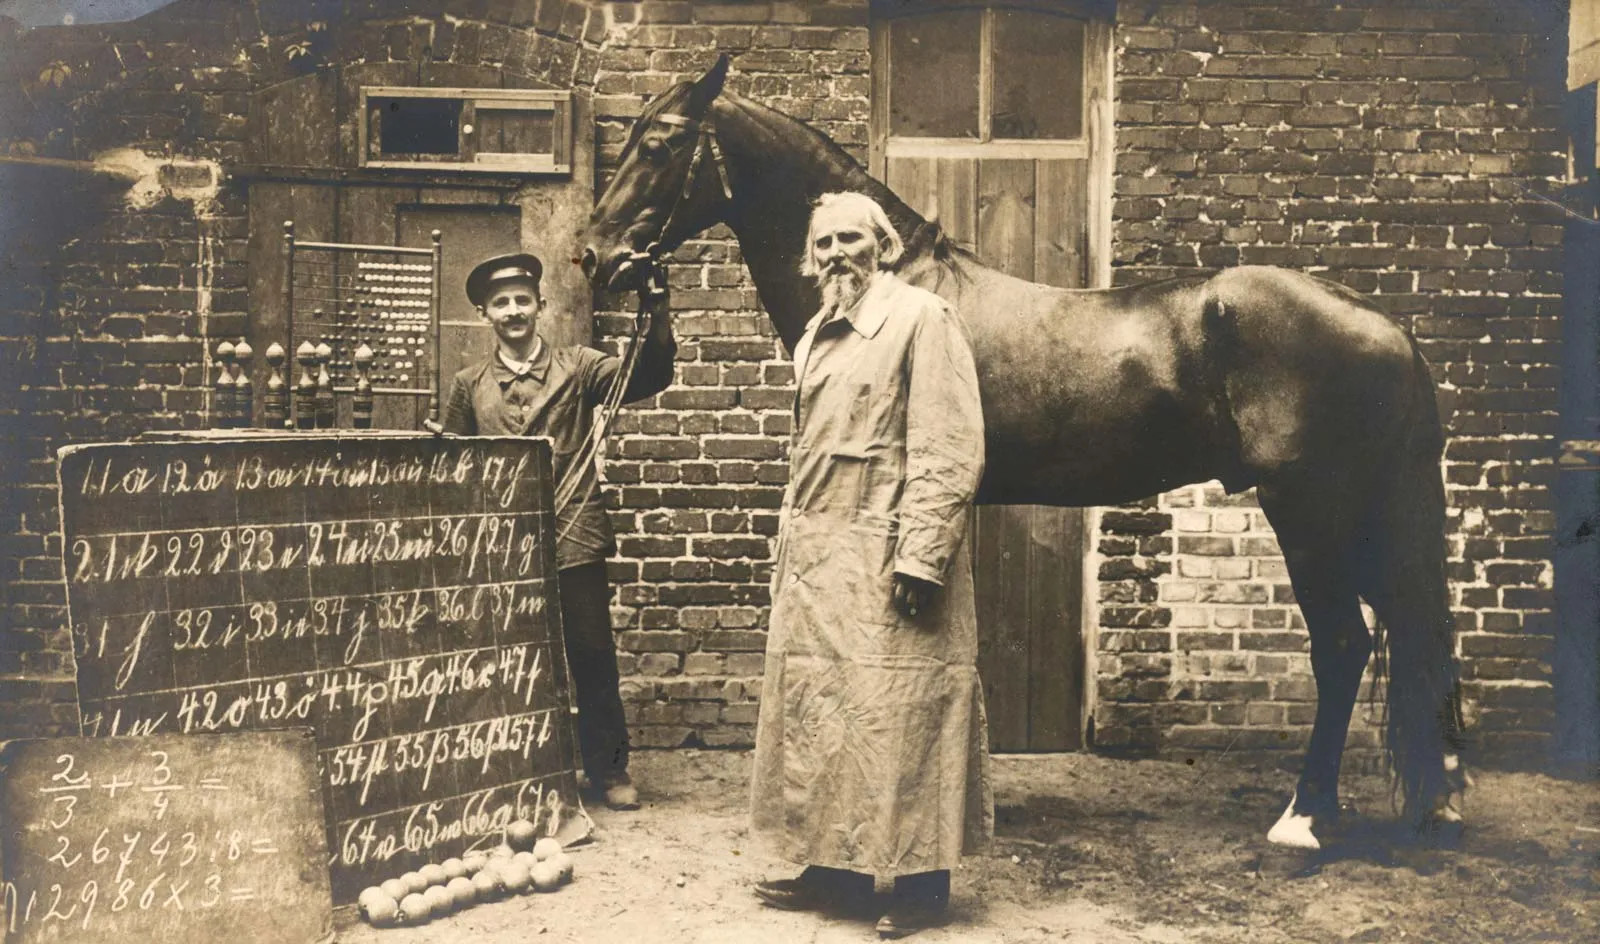
\includegraphics[width=0.6\textwidth]{images/clever-hans.jpg}
	\vspace{0.2em}

	\begin{scriptsize}
		% Send to the left S

		Source: \textit{Encyclopedia Britannica}
	\end{scriptsize}

	\pause

	\vspace{1em}
	The trainers body language was a \textit{confounding element} for the Hans arithemetic algorithm.
}

\frame{
	\frametitle{Artifacts that are possibly confounding elements}
	\centering
	\begin{figure}[ht]
		\begin{center}
			\begin{subfigure}[b]{0.3\textwidth}
				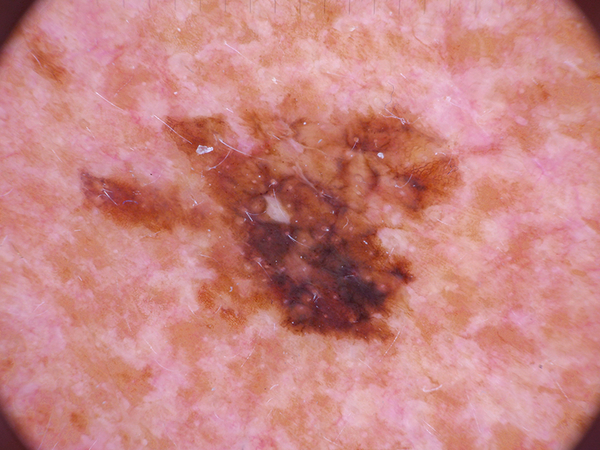
\includegraphics[width=\textwidth]{./images/ISIC_0024310.jpg}
				\caption{Image of skin lesion with black frame}
			\end{subfigure}
			\begin{subfigure}[b]{0.3\textwidth}
				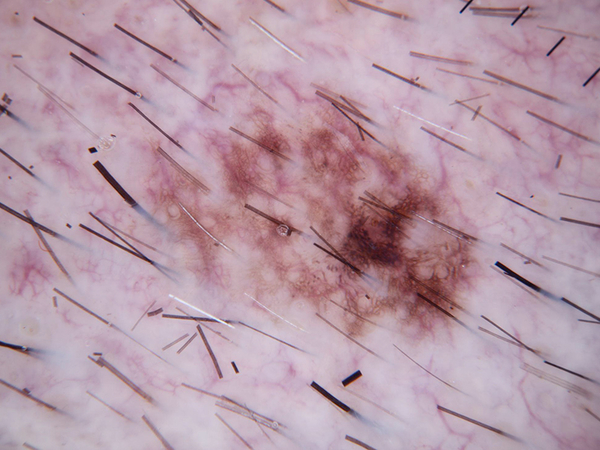
\includegraphics[width=\textwidth]{./images/ISIC_0024420.jpg}
				\caption{Image of skin lesion with ruler (upper right corner)}
			\end{subfigure}
			\begin{subfigure}[b]{0.3\textwidth}
				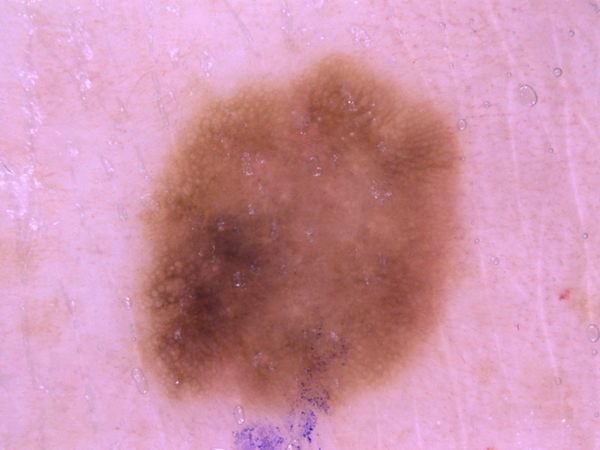
\includegraphics[width=\textwidth]{./images/ISIC_0027514.jpg}
				\caption{Image of skin lesion with blue ink}
			\end{subfigure}
		\end{center}
		\vspace{1em}
		Table 4.1

	\end{figure}

	\pause

	Data prevalence of rulers were comparatively high ($17.2\%$) - started research there.
}

\frame{
	\frametitle{Do the rulers carry relavant information?}
	\centering

	\begin{figure}[ht]

		\centering
		\includegraphics[width=0.7\textwidth]{./build/confounder_label_correlation/confusion_matrix_seaborn.png}

		\vspace{1em}
		Figure 4.2: Pivot table of rulers vs. class in the HAM10000 dataset - normalized over the x-axis.
		\label{fig:ruler_vs_dx}
	\end{figure}


}

\frame{
	\frametitle{Do the rulers carry relavant information?}
	\centering

	Thanks to Aasa for labeling the images!
}

\frame{
	\frametitle{Answer from the litterature}
	The rulers do indeed affect classification model predictions.
	I went into detail with the following two:
	\begin{itemize}
		\item (De)Constructing Bias on Skin Lesion Datasets
		\item Interpretations are useful: penalizing explanations to align neural networks with prior knowledge
	\end{itemize}
}

\frame{
	\frametitle{Original project plan}
	\begin{block}{Mission}
		Make a model that is not using the rulers as a confounding element.
	\end{block}

	\pause
	\vspace{2em}

	Plan:
	\begin{enumerate}
		\item Make a good model
		\item Show a bias
		\item Change the model
		\item Show that the model is not biased anymore
	\end{enumerate}
}

\frame{
	\frametitle{ResNet-18 Model}
	\textbf{Augmentation}: MixUp, DihedralFlip/rotation and RandomCrop
	\begin{columns}
		\begin{column}{0.4\textwidth}
			\begin{center}
				\includegraphics[width=\textwidth]{build/prediction_strength/confusion_matrix_seaborn.png}
				Figure 4.3
			\end{center}
		\end{column}
		\begin{column}{0.4\textwidth}
			\begin{table}
				\centering
				\input{build/segmented_prediction_strength/metrics_table.tex}
				\vspace{1em}

				Table 4.3: Metrics for the model as evaluated on the $20\%$ test set.
			\end{table}
		\end{column}
	\end{columns}
}

\frame{
	\frametitle{Test 1: Feature vector nearest neighbors}
	Used in "(De)Constructing Bias on Skin Lesion Datasets".
	\begin{block}{Method}
		\begin{enumerate}
			\item Choose an image with an artifact (eg. a ruler)
			\item Extract output from layers after the last convolutional layer.
			\item Find nearest neighbors of the feature vector of the image.
			\item Check if these contain the same artifact.
		\end{enumerate}
	\end{block}
	\centering
	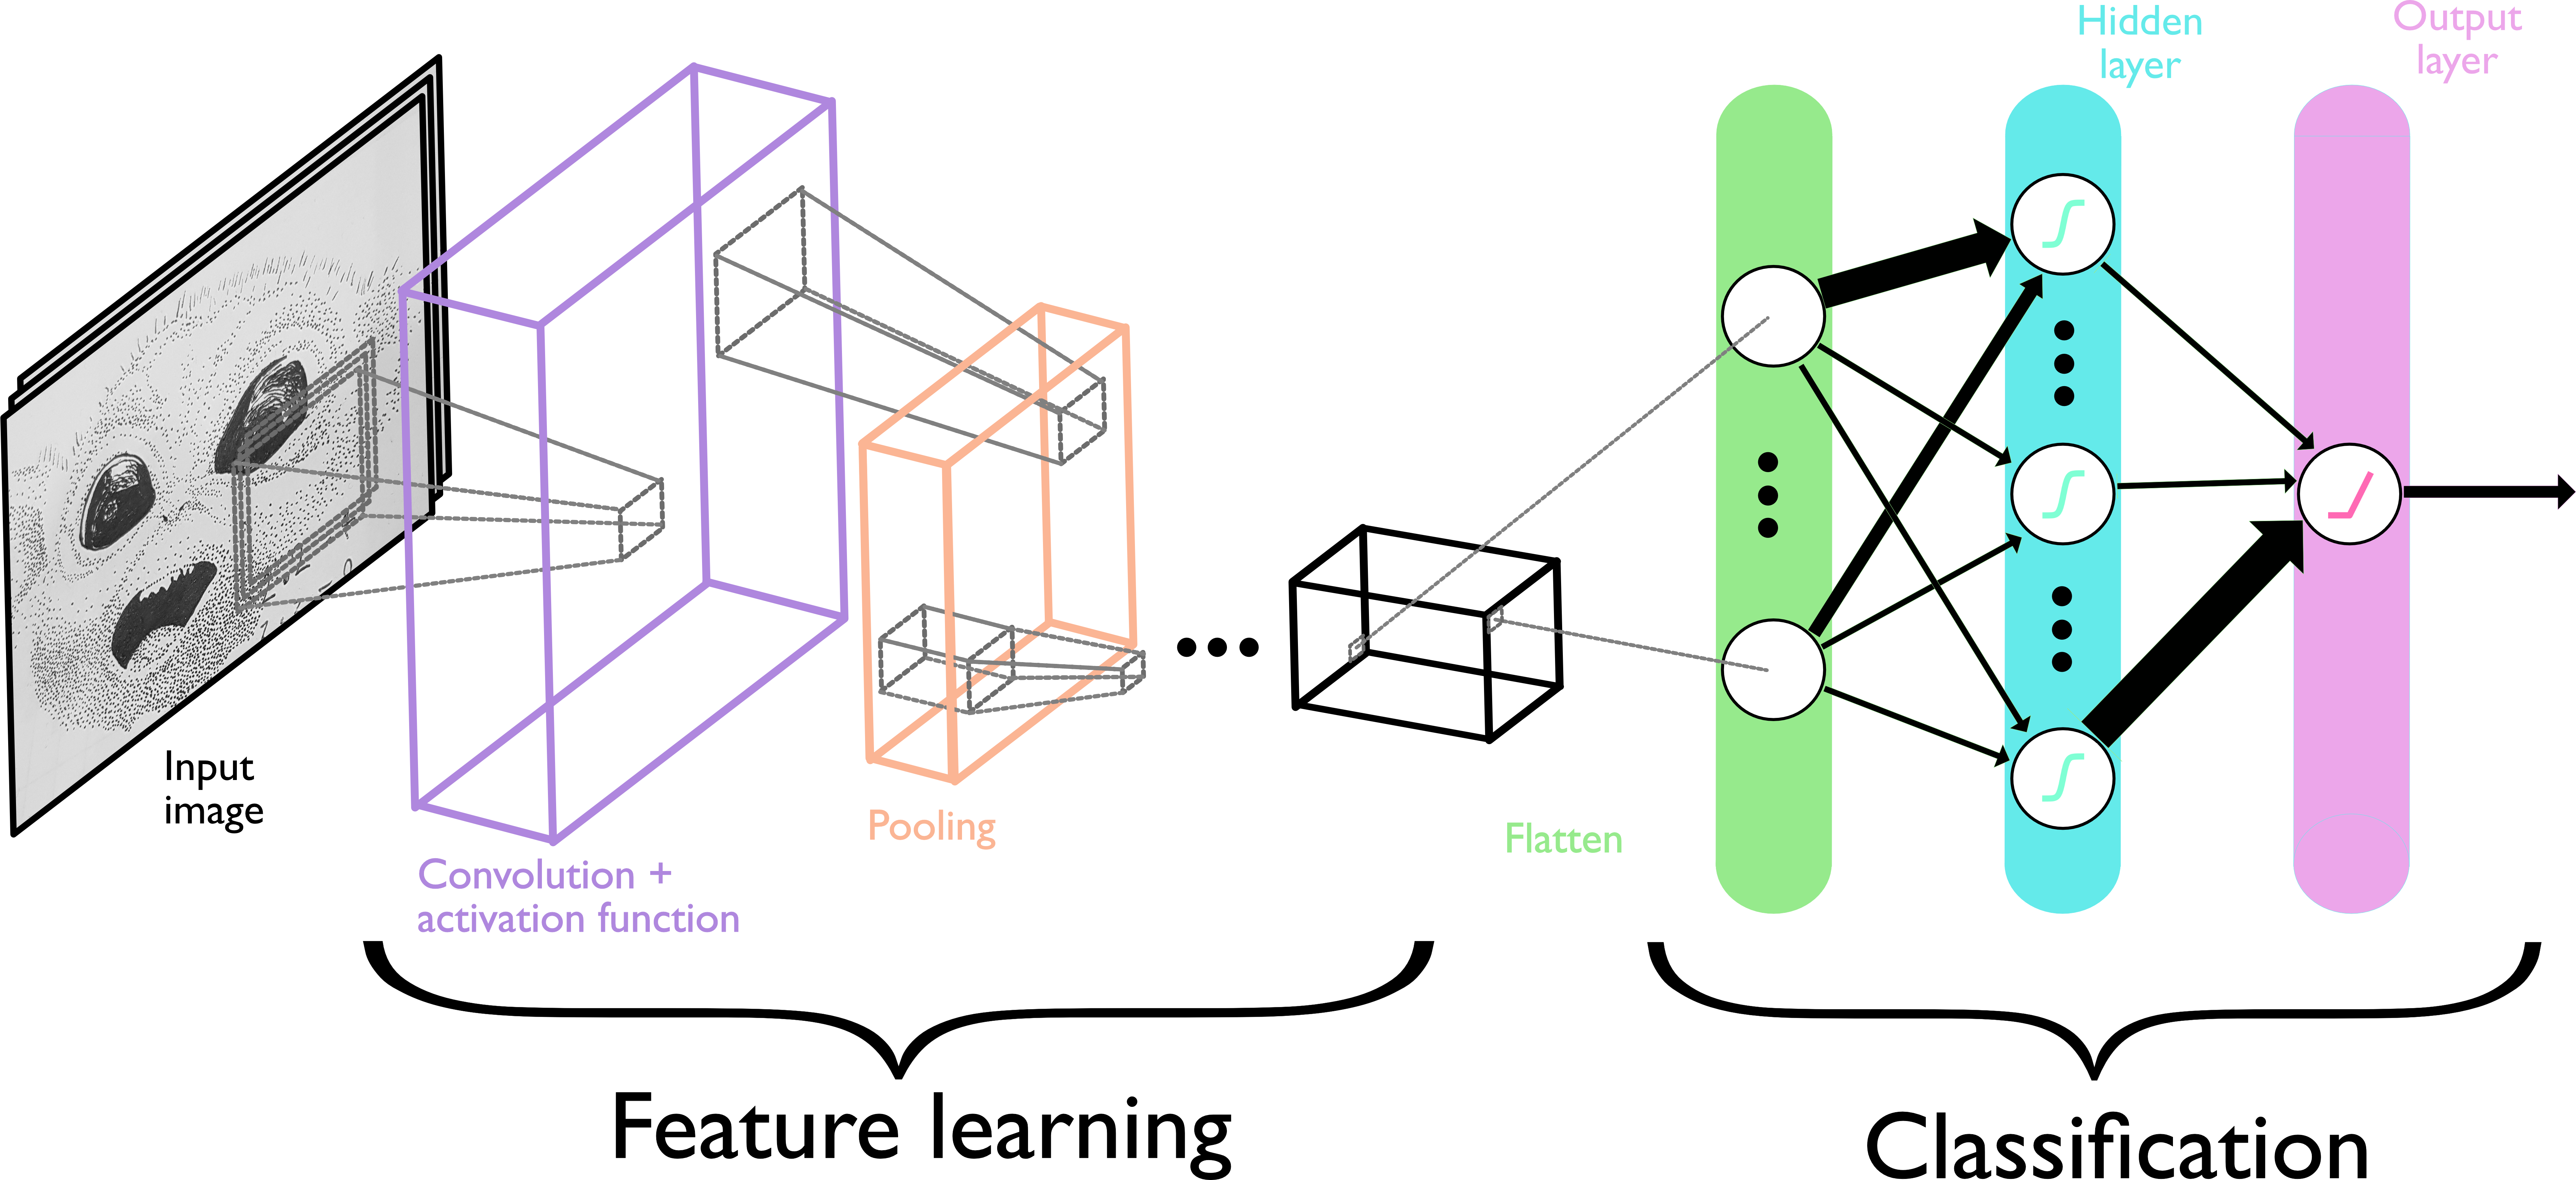
\includegraphics[width=0.4\textwidth]{images/ConvNet_V2.png}
}

\frame{
	\frametitle{Test 1: Results}
	\begin{columns}
		\begin{column}{0.3\textwidth}
			\begin{center}
				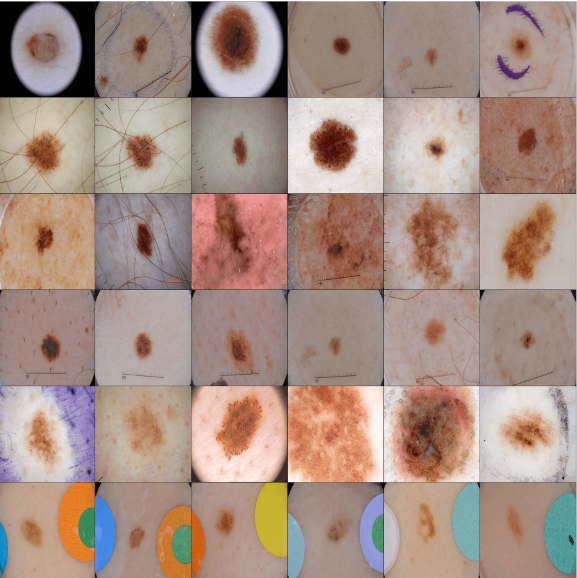
\includegraphics[width=\textwidth]{images/not-so-fast-artifact-query.png}
				Figure 2.2: Results from the paper
			\end{center}
		\end{column}
		\begin{column}{0.65\textwidth}
			\begin{center}
				\includegraphics[width=\textwidth]{build/near_neigh/examples.png}
				Figure 5.2: My results
			\end{center}
		\end{column}
	\end{columns}
}

\frame{
	\frametitle{Test 2: Saliency map}
	Method used in "Interpretations are useful: penalizing explanations to align neural networks with prior knowledge".
}

\frame{
	\frametitle{Saliency maps (an abstract definition)}
	\begin{block}{Saliency maps}
		A way to visualize the important parts of an image in relation to a models prediction.
	\end{block}

	\pause

	\textbf{Gradient based class specific}
	Utiling that if $f$ is
	\[
		f: \mathbb{R}^M \rightarrow \mathbb{R}
	\]
	where the gradient of $f$ in a point $x$ is in the vector space $\mathbb{R}^M$.

	\pause

	If $f: \mathbb{R}^{H\times W} \to \mathbb{R}$ is a clasifier and $x$ is its probability that a given image is of a certain class,
	then the gradient in $x$ is a vector that can be interpreted as an image of the same size as the input image
	\pause
	- interpretable as a \textit{saliency map}.
}

\frame{
	\frametitle{Test 2: Saliency map}
	Method used in "Interpretations are useful: penalizing explanations to align neural networks with prior knowledge".

	\begin{center}
		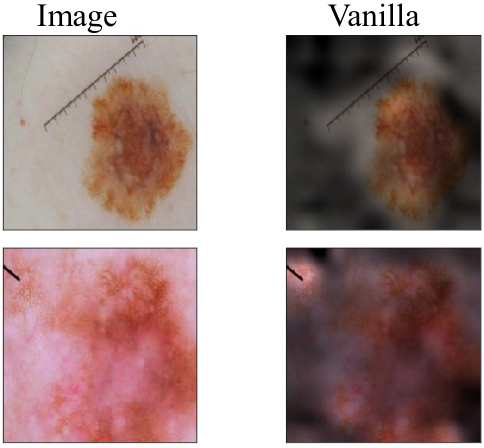
\includegraphics[width=0.4\textwidth]{images/interps-are-useful-saliency-maps.png}
	\end{center}
}

\frame{
	\frametitle{Test 2: My results}

	\begin{center}
		\includegraphics[width=\textwidth]{build/saliency_maps/overview_map_6.png}
		Figure 5.1
	\end{center}
}

\frame{
	\frametitle{Removing the ruler}

	\centering
	\includegraphics[width=0.95\textwidth]{build/segmented_images_example/segmented_images_example.png}

	\pause

	If the ruler is important to the model - it should get worse when trained on this dataset
}

\frame{
	\frametitle{Metrics for segmented model}

	\centering
	\input{build/segmented_prediction_strength/score_table.tex}

	\pause
	\vspace{2em}
	\huge

	The segmented model is better on \textit{all} metrics
}

\frame{
	\frametitle{\textit{Going back to the} Original project plan}
	\begin{block}{Mission}
		Make a model that is not using the rulers as a confounding element.
	\end{block}

	\vspace{2em}

	Plan:
	\begin{enumerate}
		\item Make a good model
		\item Show a bias \hspace{2em} \textbf{I got stuck here}
		\item Change the model
		\item Show that the model is not biased anymore
	\end{enumerate}

}


\frame{
	\frametitle{Discussion}

	\begin{itemize}
		\item Does the model use the rulers?
		      \pause
		\item Are the arguments used by other researchers solid?
		      \pause
		      \begin{itemize}
			      \item Feature vector similarity
			            \pause
			      \item Saliency maps
		      \end{itemize}
		      \pause
		\item Further research
		      \begin{itemize}
			      \pause
			      \item Making a standardized test
		      \end{itemize}
	\end{itemize}
}

\frame{
	\frametitle{Conclusion}

	\begin{itemize}
		\item The model is not using the rulers
		\pause
		\item Making the argument that a given model is using a certain artifact is very difficult
	\end{itemize}
}





\end{document}